

\documentclass[11pt]{article}
\usepackage[a4paper, total={6in,9in}]{geometry}
\usepackage[parfill]{parskip}    	
\usepackage{graphicx,caption,fancyhdr,xcolor,pdfpages,setspace}

\usepackage[hypertexnames=false]{hyperref}

\newcommand{\wrt}[1]{\mathrm{d}#1}
\newcommand{\pelahverse}{Pela\hspace*{1pt}\textbf{::}Verse}
\newcommand{\lineref}[1]{lines \textbf{#1}}

\setlength{\fboxsep}{1.5em}

\hypersetup{
	colorlinks=true,
	linkcolor=darkgray,
	citecolor=red,
	urlcolor=red
}

\urlstyle{same}
\renewcommand{\footnoterule} % Push footnotes to the bottom of the page
	{\vfill\kern -3pt \hrule width 0.4\columnwidth \kern 2.6pt}

\makeatletter
\title{\pelahverse{}: A 2D Graphical Game Powered by the Euler--Cromer Method}
\let\Title\@title
\author{Y3862181}
\let\Author\@author
\date{Summer Term, 2022}
\let\Date\@date
\makeatother

\fancypagestyle{content}{
    \renewcommand{\headrulewidth}{0.4pt}
    \renewcommand{\footrulewidth}{0.4pt}
    \setlength{\headheight}{15pt}
    
	\fancyhf{}
	\fancyhead[L]{\Author}
	\fancyhead[R]{\pelahverse{}}
	\fancyfoot[L]{\Date}
	\fancyfoot[R]{\thepage}
}
\onehalfspacing
\begin{document}
\maketitle

\begin{abstract}
\noindent
The \pelahverse{} is a two-dimensional graphical game based on an innovative concept of `space tokenomics', whereby planets are depicted as tokens capable of generating wealth if complementary tokens collide with each other. In the current prototype of this game, it is a `blue token' that needs to collide with a `yellow token' in order to gain a reward of one \textit{pelah coin}. 

In order to achieve this goal, the `blue token' needs to acquire the appropriate momentum in order to collide with the `yellow token'. The momentum of the `blue token' is determined by the gravitational force the `green token' exerts upon it and vice versa. Thus, in order to dial in the right momentum to reach the target one has to shrewdly select the initial position of the `blue token'.

In addition, obstacles (called `anti-tokens') that attempt to block the path of the `blue token' need to be implemented as well as the slick ability for all objects to bounce off the screen display. Finally, a head-up display that counts the player's current score, invigorating music and a tantalising spacey background need to be included in order to keep the customer engaged.


\end{abstract}



\section{Applying Euler--Cromer in the \pelahverse{}}
\pagestyle{content}
The first step required to meet this specification is to first learn a bit about computational physics.
\subsection{Overview of the Euler--Cromer Method}

What many physics students are not commonly taught in high school is the evident fact that analytical methods of computation, albeit elegant and efficient, are fundamentally limited. In other words, closed form solutions to a given problem is quite often insufficient when dealing with complex systems. Due to such limitations, various numerical methods have become increasingly relevant in a wide range of scientific and engineering applications. 

The reason we are discussing numerical methods in a graphical game report is simple: we will be using them! In fact, the heart of the game is based on the Euler--Cromer Method, a popular numerical method used to predict the trajectory of a body of mass in space. Figure 1 illustrates how it works. 

\begin{figure}[ht]
    \centering
    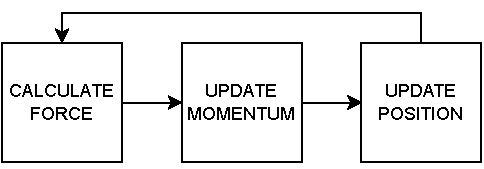
\includegraphics[width=0.5\textwidth]{Euler_Cromer.pdf}\\
    \caption{Euler--Cromer Method}
    \label{fig:Euler_Cromer}
\end{figure}

Firstly, the net force of the system needs to be calculated, which subsequently allows us to update the net momentum of the system, which finally allows us to update the instantaneous position(s) of the object(s) in the system. This is evidently an iterative process whereby its accuracy is determined by the step size of each iteration.

So how does one calculate the net force of the system? Strictly speaking it depends on the physical model we are trying to emulate. In the \pelahverse{}, luckily, we are only interested in two forces: the gravitational and spring forces embedded in the game architecture.

\subsection{The Gravitational Force}

The gravitational force is calculated by inserting values for the following equation:

\begin{equation}
    F = -\frac{G m_1 m_2}{\vert r ^ 2\vert } \hat{r}
\end{equation}	where: 

\begin{itemize}
    \item $G$ is the Gravitational Constant 6.67e-11 $(N * m^2) / kg^2)$.
    \item $m_1$ is the mass of the object that exerts a force on object 2 $(kg)$.
    \item $m_2$ is the mass of the object being affected by object 1 $(kg)$.
    \item $r$ is a vector representing the distance between the two objects $(m)$.
    \item $\hat{r}$ is the unit vector of $r$ \textit{(dimensionless)}.
\end{itemize}



This means that as long as we know the current positions and masses of each object, it should be fairly straightforward to calculate the force exerted upon them. 


\subsection{The Spring Force}

Similarly, the spring force is calculated by plugging in the values for the following equation:

\begin{equation}
    F = (L_0 - \vert(L)\vert) K \hat{L}
\end{equation}	where:

\begin{itemize}
    \item $K$ is the stiffness of the spring $(N/m)$.
    \item $L_0$ is the length of the relaxed spring $(m)$.
    \item $L$ is the vector representing the length of the compressed and rarefied spring $(m)$.
    \item $\hat{L}$ is the unit vector of $L$ (\textit{dimensionless}).
\end{itemize}


This means that as long as we know the spring stiffness, the length of the relaxed spring and the vector representing the distance between the two ends of the spring, we will be able to predict the force exerted upon it.

Since we have figured out how to calculate the gravitational and spring forces of a system, the next step is to update the net momentum of that system. This is easy. The updated net momentum is simply the previous net momentum plus the net force times the time interval between the two momenta. This can be easily illustrated using the following equation:

\begin{equation}
    p_f = p_i + F_\mathrm{net} \cdot\wrt{t}
\end{equation} where:

\begin{itemize}
    \item $p_f$ is the updated momentum.
    \item $p_i$ is the previous momentum.
    \item $F_\mathrm{net}$ is the instantaneous net force.
    \item $\wrt{t}$ is the time interval between the two momenta.
\end{itemize}

The great thing about this formula is that it applies to any system once one knows the net force exerted upon it.

Finally, we need to update the position of the object in question. This is an equally easy task since the updated position is merely the previous position plus the average instantaneous velocity (which is the instantaneous momentum of the object divided by its mass) times the time interval between the two positions. Again, this can be illustrated using the following equation:

\begin{equation} r_f = r_i + v \cdot\wrt{t} \end{equation} where:

\begin{itemize}
    \item $r_f$ is the updated position.
    \item $r_i$ is the previous position.
    \item $v$ is the instantaneous average velocity.
    \item $\wrt{t}$ is the time interval between the two positions.
\end{itemize}

And that's it! All we have to do is reiterate this process in order to successfully animate our objects in the \pelahverse{}. However, we are still unequipped to start implementing the game since we still have to find a way to convert computed values into graphics.  

\section{Allegro5 Libraries and the `Allegro Vivace' Template}

Unfortunately, our team is not competent enough to create a graphics programming environment in C from scratch, so we have to rely on a preexisting graphics programming library. The team has chosen to use Allegro5 since it enables us to achieve everything within our specification without too much difficulty.

It is possible in Allegro5 to draw primitives and fonts, animate objects, incorporate peripherals as well as import audio quite easily. What's more, Allegro5 offers a fairly thorough documentation and very useful tutorials. In fact, one of these tutorials served as the structural template of the \pelahverse\footnote {The source code for the Allegro Vivace tutorial can be found at \url{https://github.com/liballeg/allegro_wiki/wiki/Allegro-Vivace}.}.

The crew is not ashamed to admit that almost all of the functions and pointer struct data types dedicated to initialising and animating all of the custom-built objects with the aid of peripherals is taken directly from the Allegro Vivace (pronounced as Vi-Va-Ch\textit{\'{e}}) tutorial. It is in our view that if we have already imported an already-built graphics library platform, we might as well utilise a pre-existing structural template for our game design. This is precisely why we will not spend any time describing the functions and data types pertaining to the Allegro5 library or that were simply copied from the `Allegro Vivace' tutorial (see \lineref{258--331} in \hyperref[app:main-c]{\texttt{main.c}}). There are, however, a few concepts taken from that tutorial that are worth mentioning since they will greatly aid us to understand the structural intent behind the custom-built structs and functions in our program.  

The first insightful strategy our team has learnt from the `allegro vivace' tutorial was to create global structs that represent the objects described in the game specification (see \lineref{48--124} in \hyperref[app:main-h]{\texttt{main.h}}.). This way, we have the ability to assign values to any relevant parameter associated with our object at any point in our main function.

The second strategy we have mimicked from the tutorial is the use of at least three types of functions per object: initialisation, update and draw functions. \autoref{fig:Game_architecture} pretty much sums it up:

\begin{figure}[ht]
    \centering
    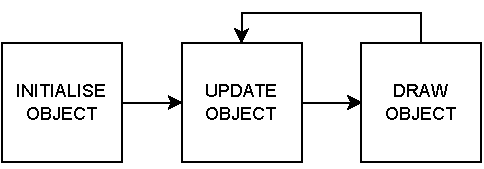
\includegraphics[width=0.5\textwidth]{Game_Architecture.pdf}
    \caption{Game Architecture}
    \label{fig:Game_architecture}
\end{figure}

Before the game starts, every parameter of each object is initialised. Then, while the game is being played, the program firstly updates each parameter for each object, and only then will these parameters be displayed. This means that every parameter of every object is pre-defined and that the program consistently maintains a clean separation between the buffer and display engine. Needless to say, the sequentially layered buffer and display engines are set up in a `while loop' configuration.


Now that we have incorporated these two elegant strategies in our game, it is time to present all of the function types for every custom-built struct in our game. 



\section{Meet the Structs and their Respective Functions}

\subsection{The Arrow}

While playing the \pelahverse{}, the `blue token' is by default attached to the tip of an object called `arrow'. The `arrow' thus enables the player to select the initial position of the `blue token' by navigating the arrow keys, which will in turn determine the initial gravitational force exerted upon it once the player hits the `space key' command.

\begin{itemize}
    \item The \texttt{arrow\_init} (see \lineref{695--705} in \hyperref[app:main-c]{\texttt{main.c}}) function initially centres the `arrow' with a magnitude of half the display height. It does not require any explicit inputs since all of the parameters are subsets of global structs. In fact, this is the case for all functions pertaining to a specified global struct in our program. 
    \item The \texttt{arrow\_update} (see \lineref{707--743} in \hyperref[app:main-c]{\texttt{main.c}}) function is a bit more interesting. It enables the player to change the magnitude and angle of the `arrow' using the arrow key commands. The nice feature about this function is that the right/left and up/down key commands independently control the angle and magnitude of the `arrow' respectively. There are also set boundaries for the magnitude of the `arrow' so that the player will not be able to set the initial position of the `blue token' on the `yellow token' itself. Finally, by pressing the space key command, the initial position of the `blue token' is determined and consequently disconnects from the tip of the arrow.  
    \item The \texttt{arrow\_draw} (see \lineref{746--755} in \hyperref[app:main-c]{\texttt{main.c}}) function draws the current state of the `arrow' onto the graphics display, but it also does one more important thing. It makes the `blue token' stick to it again once it touches its tip. This is a very useful feature since beta-testers of the program were initially frustrated that they had to fully commit to the initial position of the `blue token' once they had pressed the `space key' command. 
\end{itemize}

\subsection{The Blue Token}

This is by far the most important object in the \pelahverse{}, since it interacts with all the other objects. Careful attention to its respective functions is thus imperative for understanding the game logic design.  

\begin{itemize}
    \item The \texttt{blue\_token\_init} (see \lineref{488--504} in \hyperref[app:main-c]{\texttt{main.c}}) function does exactly what it says. The only thing that might not be obvious is that the initial position of the `blue token' is always set at the tip of the arrow function.
    \item There is an additional function to our classic `initialise, update, and draw' function suite called \texttt{blue\_token\_trigger} (see \lineref{506--515} in \hyperref[app:main-c]{\texttt{main.c}}), which basically assigns the values of the `arrow' position to the `blue token' whenever its `live' parameter state is set to `false'. This is called whenever the `blue token' touches the tip of the arrow or collides with the `yellow token' or `anti-token' objects. 
    \item The \texttt{blue\_token\_update} (see \lineref{517--592} in \hyperref[app:main-c]{\texttt{main.c}}) function is fairly extensive since it does a lot and calls other custom-built functions, which will be covered during its overall description. The first thing it does is set all the relevant parameters for prompting the Euler--Cromer Method by iteratively computing the force, momentum and position of the `blue token' for both the x and y axes using a very small step size for increased accuracy. For the Euler--Cromer Method to work properly, the unit vector for both the x and y axes are calculated with the aid of two additional local variables and a custom-built function called \texttt{vector\_mag} (see \lineref{221--228} in \hyperref[app:main-c]{\texttt{main.c}}) which computes the magnitude of a 2D vector by inputting those two local variables into it. In addition, a boundary function called \texttt{boundary} (see \lineref{244--256} in \hyperref[app:main-c]{\texttt{main.c}}) has been implemented in order to avoid a situation whereby the magnitude of the momentum of the `blue token' would end up being too high for it to be properly displayed. (The values of the boundaries have been carefully selected for the most aesthetically pleasing animation.) 
    Secondly, the function checks if the position of the `blue token' at any point in time touches the boundaries of the display. If so, the sign of its momentum parameter is flipped and hence bounces off the screen. 
    Lastly, the function checks whether the `blue token' has collided with any `anti-tokens'. This is assessed using a collision detection function called \texttt{collide} (see \lineref{230--242} in \hyperref[app:main-c]{\texttt{main.c}}), which checks whether the bounded rectangular values of one object is within the boundaries of the bounded rectangular values of another object by testing various inequalities. If the \texttt{collide} function returns \texttt{true}, the collided `anti-token' disappears and the `blue token' returns to the tip position of the arrow. \item The \texttt{blue\_token\_draw} (see \lineref{594--600} in \hyperref[app:main-c]{\texttt{main.c}}) function simply displays the current position of the `blue token'.
\end{itemize}


\subsection{The Green Token}

\begin{itemize}
    \item The \texttt{green\_token\_init} (see \lineref{604--621} in \hyperref[app:main-c]{\texttt{main.c}}) function simply initialises all the relevant parameters for the `green token'. A characteristic feature of this function is that every time it is called, the position of the `green token' is randomised using the \texttt{between} function (see \lineref{209--213} in \hyperref[app:main-c]{\texttt{main.c}}).
    \item The \texttt{green\_token\_update} (see \lineref{622--643} in \hyperref[app:main-c]{\texttt{main.c}}) function updates the position of the `green token' via the Euler--Cromer Method. Since we have already computed the gravitational force exerted upon the `blue token', there is no need to repeat the same procedure for the `green token' since the force exerted upon it must be of the equivalent opposite sign of the `blue token''s gravitational force (i.e. Newton's third law). Finally, the function also constantly checks whether the `green token' hits the boundaries of the display. If it does, the sign of its momentum is toggled hence the `green token' bounces off the display boundaries. 
    \item The \texttt{green\_token\_draw} (see \lineref{645--650} in \hyperref[app:main-c]{\texttt{main.c}}) function simply displays the `green token' at its current position. 
\end{itemize}


\subsection{The Anti-Token}

\begin{itemize}
    \item The \texttt{anti\_token\_init} (see \lineref{406--426} in \hyperref[app:main-c]{\texttt{main.c}}) function sets the initial values for an array of `anti-token' objects. The location of each `anti-token' object is randomised using the \texttt{between} function. At the start of the game, only three `anti-tokens' are visible and the maximum number of `anti-tokens' that can be capped at the value determined by the global constant \texttt{AT\_N} (see \lineref{70--71} in \hyperref[app:main-h]{\texttt{main.h}}). 
    \item The \texttt{anti\_token\_update} (see \lineref{428--467} in \hyperref[app:main-c]{\texttt{main.c}}) function uses the spring force version of the Euler--Cromer Method to animate the positions of the `anti-tokens'. In addition, the function constantly checks whether any `anti-token' collides with the boundaries of the display and if so, that particular `anti-token' will bounce off the screen. 
    \item The \texttt{anti\_token\_draw} (see \lineref{469--484} in \hyperref[app:main-c]{\texttt{main.c}}) function merely displays every `anti-token' that is currently in the `visible' state. 
\end{itemize}
 

\subsection{The Yellow Token}

\begin{itemize}
    \item The \texttt{yellow\_token\_init} (see \lineref{654--660} in \hyperref[app:main-c]{\texttt{main.c}}) function sets the initial values of all the parameters of the `yellow token'. The position of the `yellow token' is randomised whenever the function is called. 
    \item The \texttt{yellow\_token\_update} (see \lineref{662--686} in \hyperref[app:main-c]{\texttt{main.c}}) function checks whether `blue token' is colliding with it using the \texttt{collide} function. If it does collide, the `green token' is initialised to a new random position, a new `anti-token' object is generated and the `blue token' returns to the tip position of the arrow. Of course, the player also receives one \textit{pelah coin} for successfully hitting the target.
    \item The \texttt{yellow\_token\_draw} (see \lineref{688--693} in \hyperref[app:main-c]{\texttt{main.c}}) displays the current position of the `yellow token'
\end{itemize}


\section{Auxiliary Functions}

This is where the elegance of the game design goes downhill. No more tripartite function types are implemented since we are done with describing the functions pertaining to our custom structs. The \pelahverse{}, however, would not be what it is without them, so it is worth describing them for completeness. 

\begin{itemize}
    \item The \texttt{score\_init} (see \lineref{335--342} in \hyperref[app:main-c]{\texttt{main.c}}) function initialises the score to zero using Allegro's stock `ttf' font library.
    \item The \texttt{score\_draw} (see \lineref{344--371} in \hyperref[app:main-c]{\texttt{main.c}}) function draws the player's current score while playing the game and also indicates when the time is up with a final score display. It also exits when a defined frame number had been reached. 
    \item The \texttt{instruction\_draw} (see \lineref{373--402} in \hyperref[app:main-c]{\texttt{main.c}}) displays the instruction for the game before the game begins.
\end{itemize}


\section{Final Game Design}

It is time to explain how all of the global structs and functions are all tied up together to form a coherent game. Although the overall structure is based on the already discussed `initialise, update and draw' suite of executions, the team has decided to create two staged buffers instead of one. This will make it fairly easy to implement both a menu section and a game section without compromising the readability of the code. This will also help making it simple for a team of software engineers to add additional features to the menu if there is enough demand from their clients. 

By inspecting the final game design in \autoref{fig:final-design}, it is clear that one buffer is implemented for the menu section (\texttt{update menu}) and one buffer is dedicated for all the global structs of the game (\texttt{update objects}). Buttressed between these two buffers is a call for triggering the background music game. This ensures that the music will only play once the player has read and comprehended the instructions and pressed the `\texttt{Y}' key command to start the game. 

In the menu buffer stage, there is a conditional branching that tests whether the player inputs a 'Y' key command, 'ESC' key command or nothing at all. If the player hits the 'Y' key command, the program will trigger the background music and will enter the main buffer of the game. If the player hits the 'ESC' key command, the program will exit before the game even starts. If nothing is pressed, the program will remain in the menu buffer stage. 

In the main buffer stage, there is a conditional branching that tests whether the state of a global \texttt{bool} type called \texttt{done} will return either \texttt{true} or \texttt{false}. The \texttt{done} will return \texttt{true} if the player either presses the `ESC' key command or shortly after the game terminates. The way the latter has been implemented is by creating a global \texttt{int} data type called \texttt{frame}. \texttt{frame} increments by one whenever the main buffer undergoes a full cycle. Since it continuously increments, it is possible to determine the exact amount of time remaining for the player to play the \pelahverse\ (at least as long as the frames per second value is known). 


\begin{figure}[h!]
    \centering
    \fbox{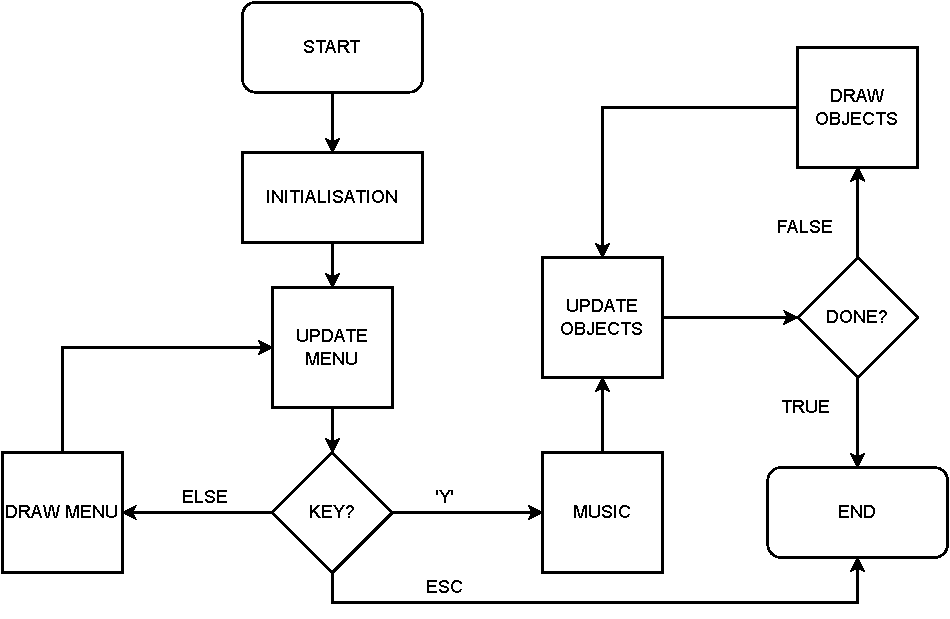
\includegraphics[width=0.8\textwidth]{final_diagram}}
    \caption{Final Game design}%
    \label{fig:final-design}
\end{figure}


\section{Evaluation}
The team have successfully implemented the specification for the game, and have even made special effort to include a header file that includes all the global structs, constants and variables as well as prototype functions for improved readability and extensibility. There are, however, certain aspects about the game and its implementation that need improvement.

Firstly, the fact that there are only two objects, which have a gravitational force exerted upon them degrades the quality of the user experience. It would have been better if, for instance, the `anti-tokens' would have had an additional effect on the updated trajectory of the `blue token' and `green token'. What's more, some functions (e.g. \texttt{blue\_token\_update}) could have been more compact to increase the modular nature and efficiency of the program. 

Another fundamental drawback is that since this game is a physics based one, there are certain values such as the Gravitational Constant that forces the team to use a lot of \texttt{double} data types, which might use a bigger memory footprint than \texttt{int} and \texttt{float} data types.

Finally, it could have been a good idea to create a global struct for the $x$-  and $y$-coordinates of the objects. This way, the code would have been more readable since the Euler--Cromer Method would only be called once instead of twice per render. What's more, if requested by future clients, it would make it easier to upgrade the game into a 3D display by simply appending a $z$-coordinate onto the struct.

\vfill
\begin{figure}[h!]
    \centering
    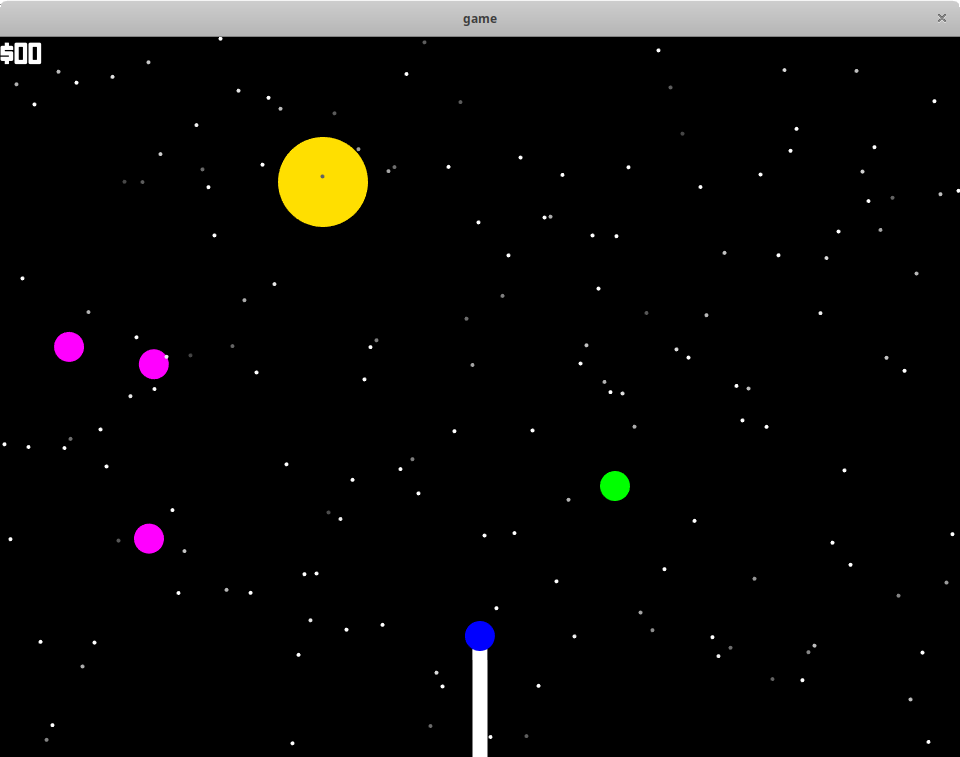
\includegraphics[width=.6\textwidth]{game-screenshot.png}\\[1em]
    \caption*{\hspace*{4pt}\Large\pelahverse}
\end{figure}
\vfill

\clearpage
\appendix

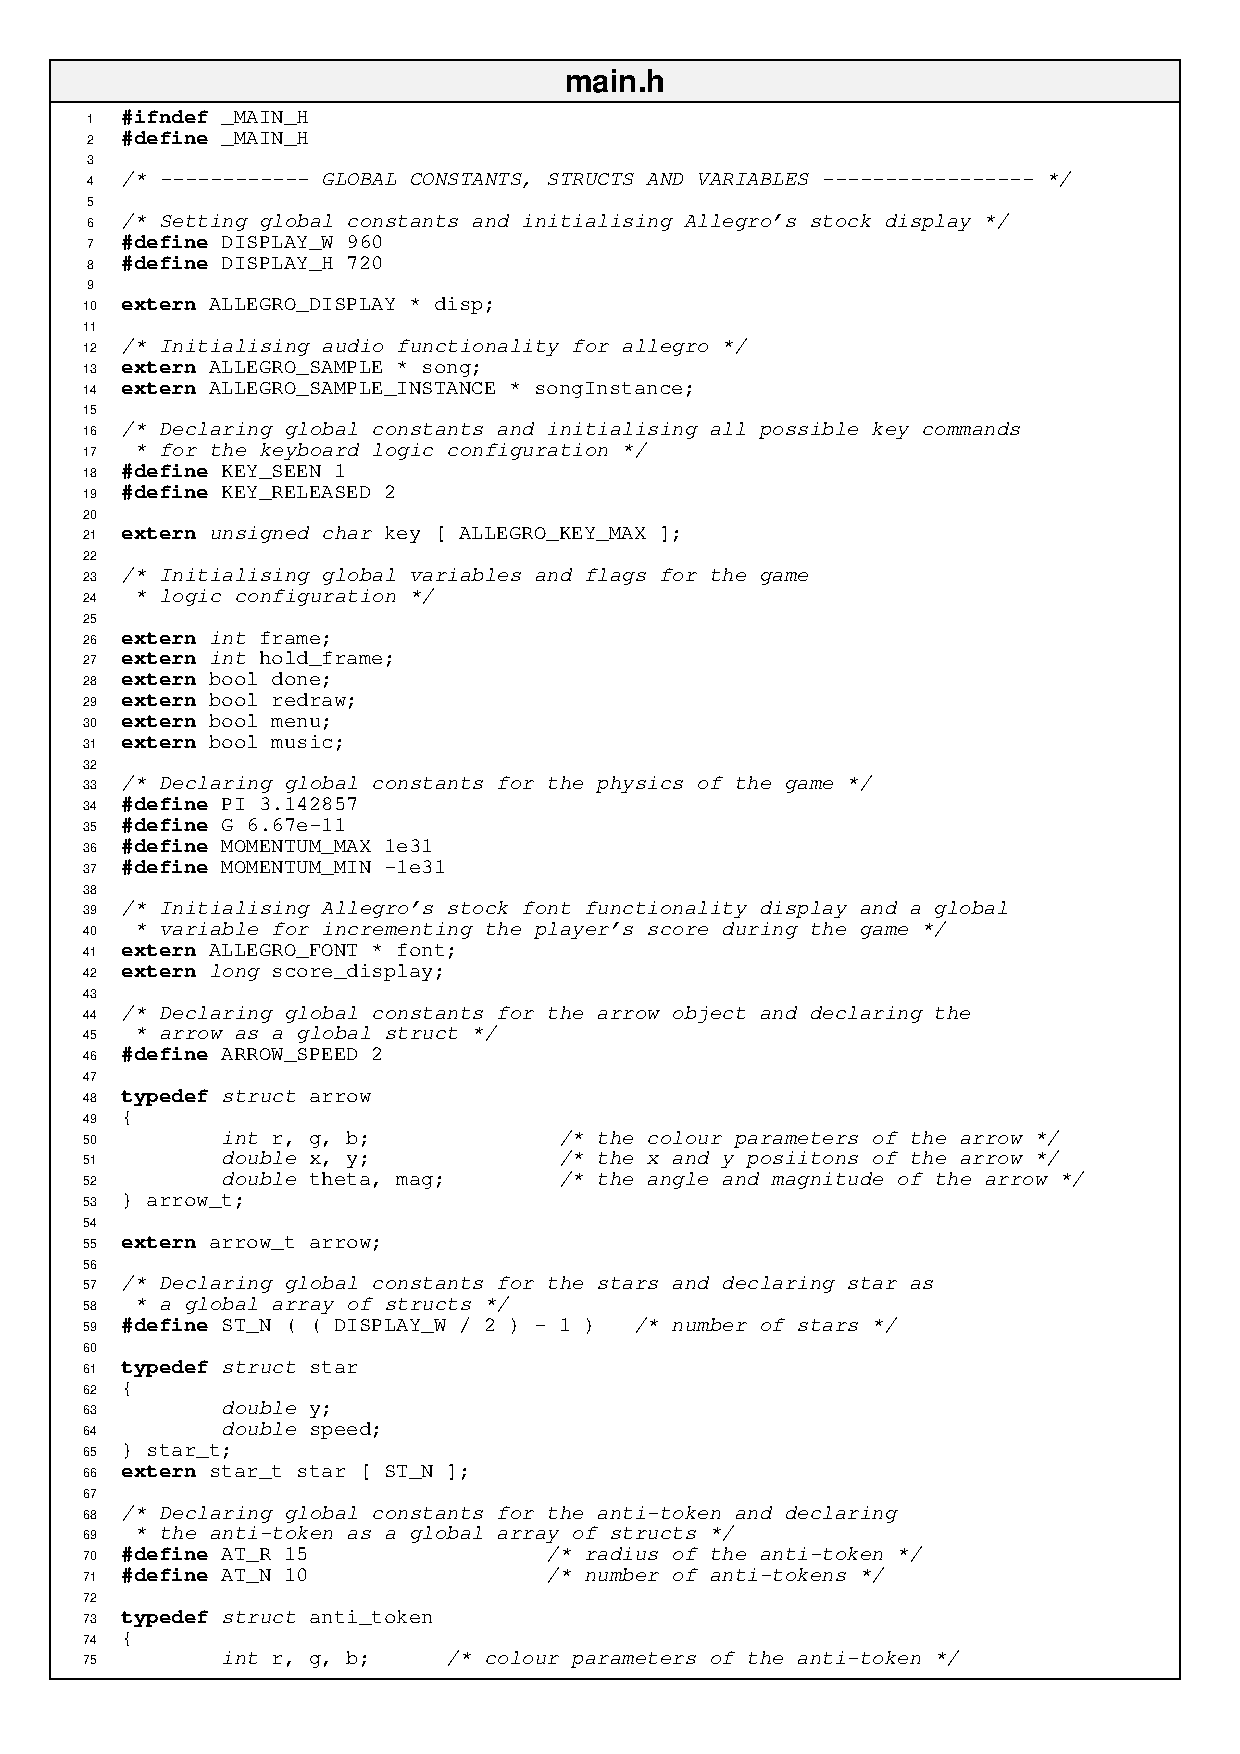
\includepdf[pages=1,pagecommand=\thispagestyle{content}%
    \section{Source Code Listing}\label{app:main-h},scale=0.8,%
    offset=0 4]{main_h.pdf}
\includepdf[pages=2-,pagecommand=\thispagestyle{content},%
    scale=0.8,offset=0 20]{main_h.pdf}

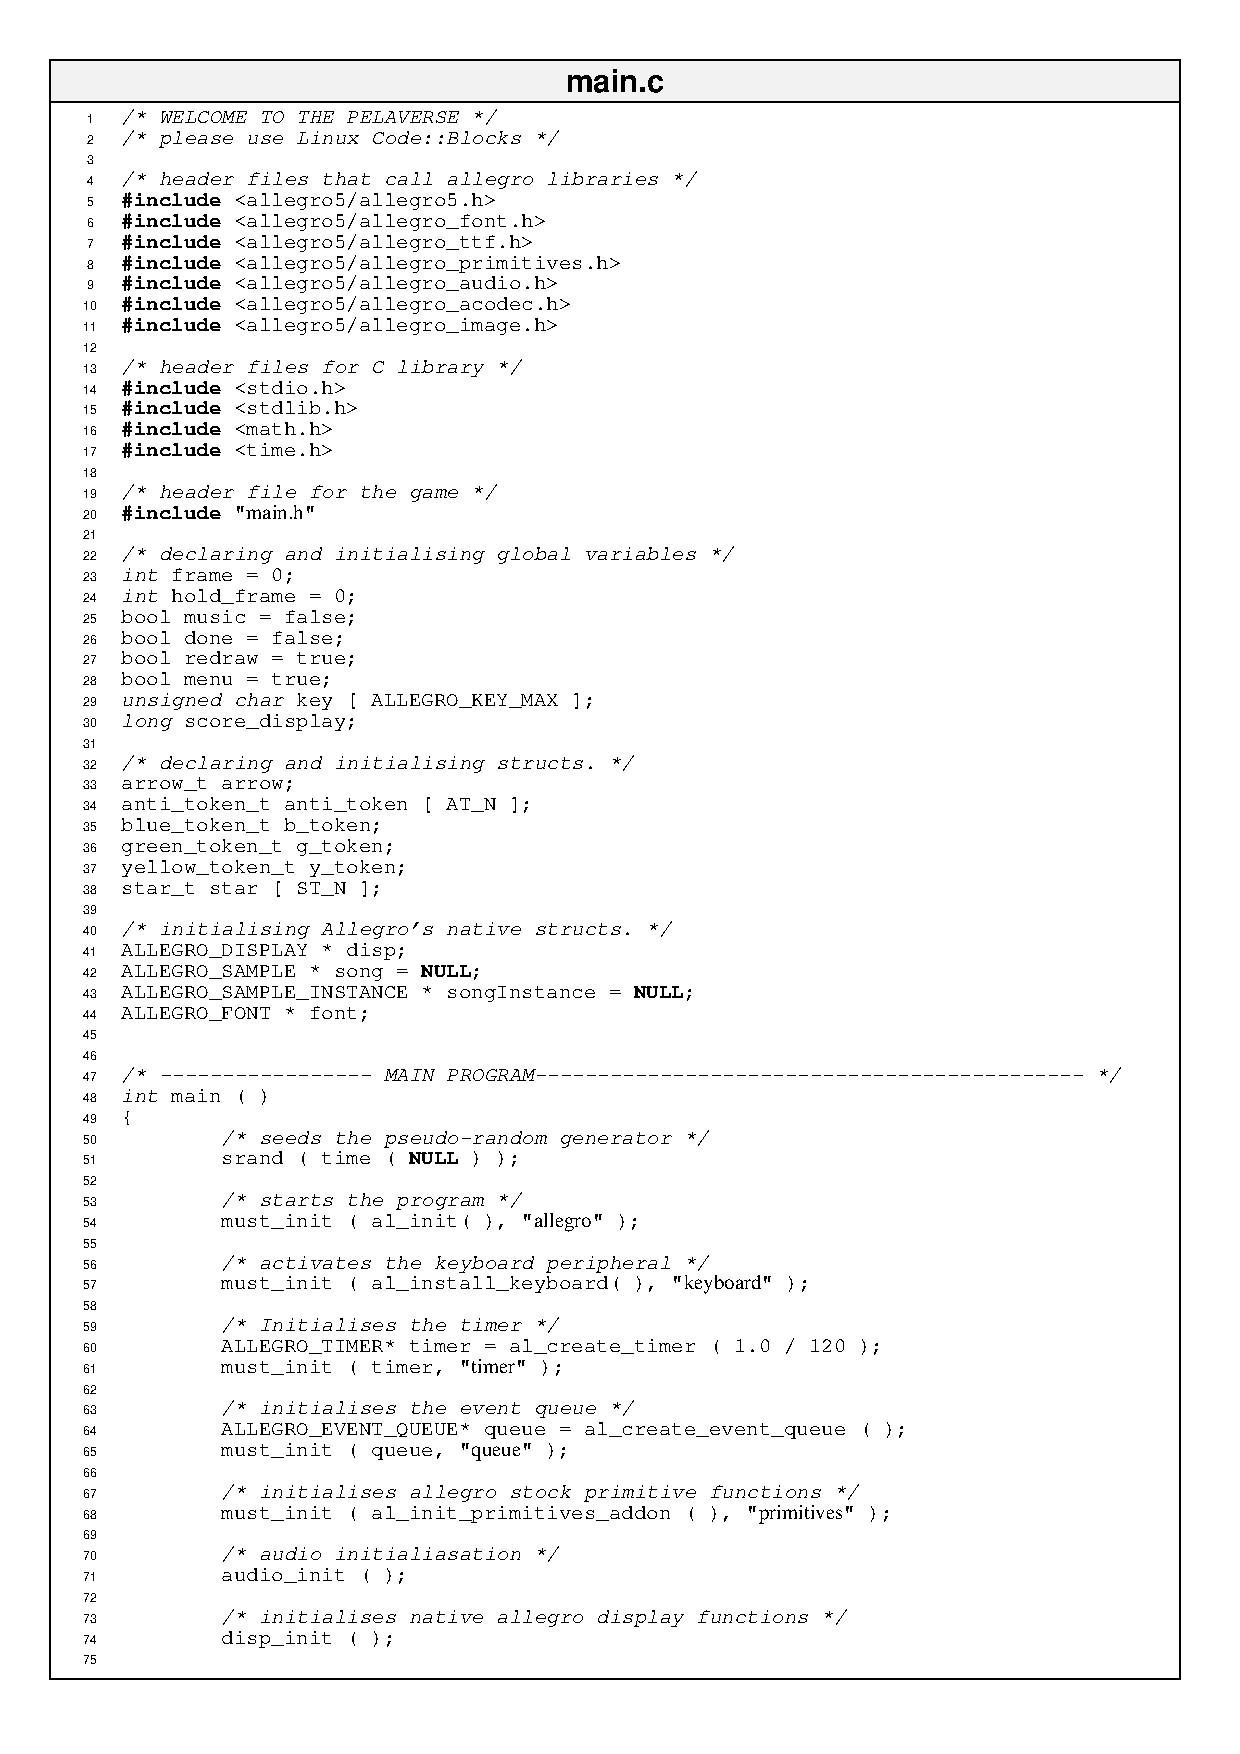
\includepdf[pages=1,pagecommand=\thispagestyle{content}%
    \refstepcounter{section}\label{app:main-c},scale=0.8,offset=0 20]{main_c.pdf}
\includepdf[pages=2-,pagecommand=\thispagestyle{content},%
    scale=0.8,offset=0 20]{main_c.pdf}

\end{document}  